\documentclass[9pt]{beamer}

% --- Packages ---
\usepackage{amsmath, amssymb}

% (Optional) compile with XeLaTeX/LuaLaTeX for fonts
\usepackage{fontspec}
\setmainfont{Times New Roman}
\usepackage{unicode-math}

\usepackage{tikz}
\usetikzlibrary{arrows.meta, positioning, decorations.pathreplacing, calc, fit, backgrounds, patterns}

\setbeamertemplate{footline}[frame number]
\setbeamertemplate{navigation symbols}{}
\setbeamertemplate{caption}{\insertcaption}

% color shorthands
\definecolor{accent}{RGB}{0,90,160}
\definecolor{invest}{RGB}{200,70,30}
\definecolor{shockc}{RGB}{20,140,90}

\title{Where Does the Investment Demand Shock Come From?}
\subtitle{A toy model of idiosyncratic shocks and lumpy investment}
\author{Li Xuanguang}
\date{\today}

\begin{document}

\begin{frame}
	\titlepage
	\vspace{-1em}
	\begin{center}\footnotesize Building on \textit{Nirei and Ragot (2025)}\end{center}
\end{frame}

% ==================================================
% Roadmap
% ==================================================
\begin{frame}{What this toy model is for}
	A micro-foundation that answers three questions for the estimation:
	\begin{enumerate}
		\item What do we mean by \textbf{propagation of an idiosyncratic shock}?
		\item Why is the \textbf{lumpy-investment} assumption essential?
		\item Why is it legitimate to use a \textbf{reduced-form investment demand shock}
		      (a shock added directly on investment) in estimation?
	\end{enumerate}

	\vspace{0.8em}
	\textbf{Logic of the argument:}
	\begin{itemize}\small
		\item A small i.i.d.\ shock pushes a few firms over their investment threshold.
		\item In general equilibrium this raises output, which moves \emph{every} firm's threshold.
		\item The induced wave does \textbf{not} die out — it is self-sustaining and, in the limit
		      of many firms, survives as a \textbf{degenerate (non-random) aggregate} investment shock.
	\end{itemize}
\end{frame}

% ==================================================
% 1. Intermediate goods producers
% ==================================================
\section{Setup}

\begin{frame}{Intermediate-goods producers}
	Standard New-Keynesian CES aggregator and demand:
	\[
		Y_t=\Big(\int_0^1 y_{jt}^{\frac{\eta-1}{\eta}}\,dj\Big)^{\frac{\eta}{\eta-1}},
		\qquad
		y_{jt}=\Big(\frac{p_{jt}}{P_t}\Big)^{-\eta}Y_t,
		\qquad
		y_{jt}=a_{jt}k_{jt}.
	\]
	Linear-in-capital technology $y_{jt}=a_{jt}k_{jt}$. Combining demand and production, real revenue is
	\[
		r_{jt}(a_{jt},k_{jt})=\frac{p_{jt}y_{jt}}{P_t}
		=\big(a_{jt}k_{jt}\big)^{1-\frac1\eta}\,Y_t^{\frac1\eta}.
	\]
	\begin{itemize}\small
		\item Concave in own capital ($\eta>1$): diminishing returns through the demand curve.
		\item Revenue, hence the desired capital, scales with aggregate output $Y_t$ — the channel
		      through which one firm's action will later spill over to all firms.
	\end{itemize}
\end{frame}

% ==================================================
% 2. Lumpy investment & value function (Figure 1)
% ==================================================
\section{Lumpy investment}

\begin{frame}{Lumpy investment and the investment threshold}
	% --- top region: text (left) + figure pinned NE (right) ---
	\begin{columns}[T]
		\column{0.56\textwidth}
		Firms solve
		\[\small
			\max_{\{x_{t+k}\}}\ \mathbb{E}_t\!\sum_{k\ge0}\Lambda_{t,t+k}\big(r_{j,t+k}-x_{j,t+k}\big),
		\]
		$$\begin{aligned}
			\text{s.t. }&k_{j,t+1}=(1-\delta)k_{j,t}+x_{j,t},\\
			&x_{j,t+k}\in\{0,\ \lambda k_{j,t+k}\}.
		\end{aligned}$$

		\column{0.44\textwidth}
		\vspace{-0.6em}
		\centering
		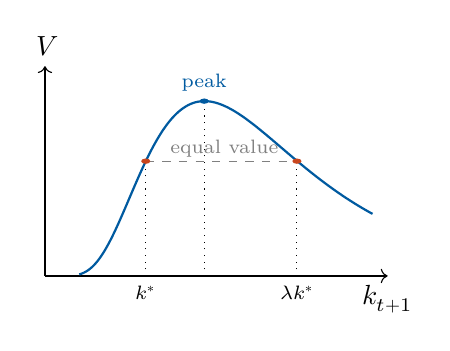
\begin{tikzpicture}[xscale=1.28,yscale=0.74]
			% axes
			\draw[->] (0,0) -- (3.4,0) node[below]{$k_{t+1}$};
			\draw[->] (0,0) -- (0,3.6) node[above]{$V$};
			% hump: peak at sqrt(lambda)*k*, k*=1, lambda=2.5 -> peak 1.58
			\draw[thick,accent,domain=0.34:3.25,samples=140,smooth,variable=\x]
				plot ({\x},{3*exp(-2*(ln(\x)-0.459)^2)});
			% equal-value horizontal line between k* and lambda k*
			\draw[dashed,gray] (1,1.97) -- (2.5,1.97);
			\draw[dotted] (1,0) -- (1,1.97);
			\draw[dotted] (2.5,0) -- (2.5,1.97);
			\draw[dotted] (1.58,0) -- (1.58,3.0);
			% points
			\fill[invest] (1,1.97) circle (1.3pt);
			\fill[invest] (2.5,1.97) circle (1.3pt);
			\fill[accent] (1.58,3.0) circle (1.3pt);
			% x ticks
			\node[below,font=\scriptsize] at (1,0) {$k^{*}$};
			\node[below,font=\scriptsize] at (2.5,0) {$\lambda k^{*}$};
			\node[above,font=\scriptsize,accent] at (1.58,3.0) {peak};
			\node[font=\scriptsize,gray] at (1.78,2.18) {equal value};
		\end{tikzpicture}
	\end{columns}

	% --- bottom region: full-width text wrapping under the figure ---
	\vspace{0.3em}
	Indifference at $k^*$ (the firm knows its next-period technology) pins down the threshold:
	\[
		k_{j,t+1}^{*}=a_{j,t+1}^{\,\eta-1}\,\Phi_t(\Lambda_t, \Lambda_{t+1})\,Y_{t+1}\,
	\]
	\begin{itemize}\small
		\item Desired capital scales with aggregate output $Y_{t+1}$ — the spillover channel that will carry one firm's action to all firms.
	\end{itemize}
	\vspace{0.4em}
	Normalize a firm's position by its \textbf{distance to the threshold}
	\[
		s_{jt}=\frac{\log\!\big(k_{jt}/k_{jt}^{*}\big)}{\log\lambda},
	\]
	so that investing means jumping up exactly one notch ($s\mapsto s+1$) in these units.
\end{frame}


% ==================================================
% 3. Stationary distribution & investing fraction (Figure 2)
% ==================================================
\section{Stationary distribution}

\begin{frame}{Cross-section stationary distribution}
	% --- top region: text (left) + figure pinned NE (right) ---
	\begin{itemize}
		\item Assume $a_t\in\{a_L,a_H\}$ and $s_t\mid a_t\sim U[0,1)$ under stationary distribution.
		\item Macro variables are constant: $Y = Y_t = Y_{t+1}$, $\Phi = \Phi_t = \Phi_{t+1}$
	\end{itemize}

	\begin{columns}[T]
		\column{0.5\textwidth}
		
		Without investing, position drifts by
		\[
		\begin{aligned}
		s_{j,t+1}&=s_{j,t}(a) \\
		&-\underbrace{\frac{-\log(1-\delta)+(\eta-1)\log\frac{a'}{a}}{\log\lambda}}_{s^{*}(a,a')}.
		\end{aligned}
		\]

		\column{0.5\textwidth}
		\centering
		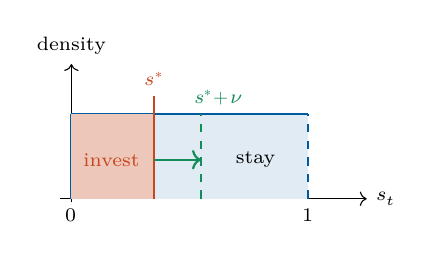
\begin{tikzpicture}[xscale=3.0,yscale=0.9]
			% axis
			\draw[->] (-0.05,0) -- (1.25,0) node[right,font=\scriptsize]{$s_t$};
			\draw[->] (0,-0.05) -- (0,1.9) node[above,font=\scriptsize]{density};
			% uniform density box on [0,1)
			\fill[accent!12] (0,0) rectangle (1,1.2);
			\draw[accent,thick] (0,1.2) -- (1,1.2);
			\draw[accent,thick] (0,0)--(0,1.2);
			\draw[accent,thick,dashed] (1,0)--(1,1.2);
			% investing region [0,s*]
			\fill[invest!30] (0,0) rectangle (0.35,1.2);
			\draw[invest,thick] (0.35,0)--(0.35,1.45);
			\node[invest,font=\scriptsize,above] at (0.35,1.45) {$s^{*}$};
			% epsilon shifted threshold
			\draw[shockc,thick,->] (0.35,0.55)--(0.55,0.55);
			\draw[shockc,thick,dashed] (0.55,0)--(0.55,1.2);
			\node[shockc,font=\scriptsize,above] at (0.62,1.18) {$s^{*}\!+\!\nu$};
			% labels
			\node[invest,font=\scriptsize] at (0.17,0.55) {invest};
			\node[font=\scriptsize] at (0.78,0.55) {stay};
			\node[below,font=\scriptsize] at (0,0) {$0$};
			\node[below,font=\scriptsize] at (1,0) {$1$};
		\end{tikzpicture}
	\end{columns}

	% --- bottom region: full-width text wrapping under the figure ---
	\vspace{0.em}
	\begin{itemize}
		\item Since $s_t\sim U[0,1)$, $s^{*}(a,a')$ is the \textbf{investing fraction}
		\item Add an i.i.d.\ shock $\varepsilon$ on $a'$ \emph{only} in group $(a,a')=(b,b')$:
		\[\small
			s^{*}(b,\varepsilon b')=s^{*}(b,b')+\underbrace{\frac{(\eta-1)\log\varepsilon}{\log\lambda}}_{\nu}.
		\]
		\item The cutoff in that group rises by $\nu$, so an extra $\nu$-mass invests.
	\end{itemize}
\end{frame}

% ==================================================
% 4. Idiosyncratic shock & propagation (Figure 3)
% ==================================================
\section{Idiosyncratic shock \& propagation}

\begin{frame}{An idiosyncratic shock in one group}
	% --- top region: text (left) + figure pinned NE (right) ---
	\begin{columns}[T]
		\column{0.6\textwidth}
		

		\column{0.4\textwidth}
		\vspace{-0.6em}
		\centering
		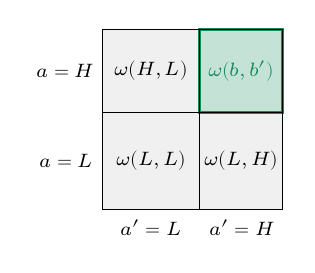
\begin{tikzpicture}[scale=0.88]
			% 2x2 groups, sizes ~ omega
			\fill[gray!12] (0,0) rectangle (1.4,1.4);
			\fill[gray!12] (1.4,0) rectangle (2.6,1.4);
			\fill[gray!12] (0,1.4) rectangle (1.4,2.6);
			% highlight shocked group (b,b'): a=H (top), a'=H (right)
			\fill[shockc!25] (1.4,1.4) rectangle (2.6,2.6);
			\draw[shockc,very thick] (1.4,1.4) rectangle (2.6,2.6);
			% grid
			\draw (0,0) rectangle (2.6,2.6);
			\draw (1.4,0)--(1.4,2.6);
			\draw (0,1.4)--(2.6,1.4);
			% labels of omega
			\node[font=\scriptsize] at (0.7,0.7) {$\omega(L,L)$};
			\node[font=\scriptsize] at (2.0,0.7) {$\omega(L,H)$};
			\node[font=\scriptsize] at (0.7,2.0) {$\omega(H,L)$};
			\node[font=\scriptsize,shockc] at (2.0,2.0) {$\omega(b,b')$};
			% axis labels
			\node[below,font=\scriptsize] at (0.7,0) {$a'=L$};
			\node[below,font=\scriptsize] at (2.0,0) {$a'=H$};
			\node[left,font=\scriptsize] at (0,0.7) {$a=L$};
			\node[left,font=\scriptsize] at (0,2.0) {$a=H$};
		\end{tikzpicture}
		\\[0.1em]
		{\scriptsize Figure 3. Four groups $(a,a')$ with masses
		$\omega$; the shock hits group $(b,b')$.}
	\end{columns}

	% --- bottom region: full-width text wrapping under the figure ---
	\vspace{0.3em}
	More investment in $(b,b')$ raises \emph{future aggregate output}:
	\[\small
		Y_{t+1}(b,b',\nu)=\Big(\omega(b,b')\!\!\int_0^1\!\! \big(b'k_{t+1}(s_t)\big)^{\frac{\eta-1}{\eta}}\,dF(s_t\mid b)\Big)^{\frac{\eta}{\eta-1}},
	\]
	split at the cutoff $s^{*}(b,b')+\nu$ into investing firms and the rest. This output increase is \textbf{propagation}.
\end{frame}

\begin{frame}{Propagation through the threshold, and why it does not die out}
	Higher $Y_{t+1}$ raises $k^{*}\propto Y_{t+1}$ everywhere, shifting the cutoff in \emph{every} group:
	\[
		s^{*}_t(a,a',\nu)=\frac{-\log(1-\delta)+(\eta-1)\log(a'/a)+\log Y_{t+1}(\nu)-\log Y_t}{\log\lambda}.
	\]
	Per-group and aggregate \textbf{$\nu$-induced fraction}:
	\[
		\Delta s^{*}_t(a,a',\nu)=\frac{\log Y_{t+1}(\nu)-\log Y_t}{\log\lambda},
		\qquad
		\Delta s^{*}_t(\nu)=\sum_{(a,a')}\omega(a,a')\,\Delta s^{*}_t(a,a',\nu).
	\]
	\begin{itemize}\small
		\item The first $\nu$ of investing firms raises $Y$, which induces $\Delta s^{*}(\nu)$ more, which raises $Y$ again $\dots$ a GE multiplier that iterates to a new equilibrium.
		\item Key theoretical property (small-shock limit):
		\[
		 \lim_{\nu\to0}\frac{\Delta s^{*}_t(\nu)}{\omega(b,b')\,\nu}=1\
		\]
		the $\nu$-induced fraction has the \emph{same scale} as the original $\varepsilon$-induced fraction $\Rightarrow$ the wave does \textbf{not} attenuate across iterations.
	\end{itemize}
\end{frame}

% ==================================================
% 5. Macro-level investment shock
% ==================================================
\section{From micro to macro}

\begin{frame}{Why a reduced-form macro investment demand shock is justified}
	\textbf{The tension.} At each iteration more firms invest, but each adds only a small amount; if the per-firm amount decayed fast enough, aggregate investment would barely move.
	$$\text{Total investment} = \sum_{i=1}^{\infty} \text{ induced investing fraction}^{i} \times \text{ average investment}^{i}$$
	\vspace{0.4em}
	\textbf{Where lumpiness bites.} With lumpy investment, ``if you invest, you must invest a large amount'' ($x=\lambda k$). The fraction result above ($\lim=1$) keeps the \emph{mass} of investors from shrinking, and lumpiness keeps each contribution \emph{large}.

	\vspace{0.6em}
	\begin{block}{Theoretical result}
		As the number of firms $\to\infty$, the i.i.d.\ idiosyncratic shock $\varepsilon$ vanishes with \textbf{asymptotic variance to zero}, yet the induced aggregate investment converges to a \textbf{non-degenerate random variable}.
	\end{block}

	\vspace{0.4em}
	\textbf{Implication for estimation.} The micro idiosyncratic shock aggregates into a well-defined, non-vanishing movement in \textbf{investment}. So it is legitimate to model it as a reduced-form shock placed \textbf{directly on investment}, rather than on technology.
\end{frame}

\begin{frame}{Takeaways}
	\begin{enumerate}
		\item \textbf{Propagation} $=$ a within-group idiosyncratic shock raising aggregate output, which feeds back onto every firm's investment threshold.
		\item \textbf{Lumpy investment} is essential: it creates the threshold (the investing fraction $s^{*}$) and guarantees each induced investment is large, so the aggregate effect does not wash out.
		\item \textbf{Reduced-form ID shock} is justified: the aggregated micro shock survives as a degenerate shock on investment, validating adding it directly to investment in estimation.
	\end{enumerate}
\end{frame}

\end{document}
